\chapter{An application of Hawkes process}
\label{chapter:application}
In reality, a Hawkes processes have been applied in many areas from earthquake to financial analysis. In this chapter, we introduce an application of Hawkes process in seismology.\\
In the 1970s, professor Alan Hawkes introduced a mathematical model of self-exciting process in seismology, which is called Hawkes process. And then it was expanded by Y.Ogata and L.Adamopoulos. In \autoref{figure:earth} illustrates the number of shocks in periods of three months for an area of the North Atlantic as same as the stochastic intensity function of a Hawkes process. Therefore, the ETAS model was introduced to modeling the earthquake times and magnitudes \cite{thesis}. They are given as follows:
\begin{align*}
	\lambda(t) = \lambda_0 + \alpha \sum_{T_i < t}e^{\beta \kappa_i}e^{-\delta(t - T_i)},
\end{align*}
where $\kappa_i \in [0, \infty)$ is the magnitude of an earthquake occurring at time $T_i$ and $\alpha , \beta, \delta > 0$ are parameters. In case 
\begin{align*}
	f(\kappa| t) = \gamma e^{-\gamma t}
\end{align*}
Additional, we can define it by its conditional intensity function including both marks and times
\begin{align*}
	\lambda(t, \kappa) = (\lambda_0 + \alpha \sum_{T_i < t}e^{\beta \kappa_i}e^{-\delta(t - T_i)})\gamma e^{-\gamma t}
\end{align*}  
The idea of this model is that earthquakes cause aftershocks, large earthquakes increase the intensity more than small earthquakes. 
\begin{figure}[H]
	\centering
	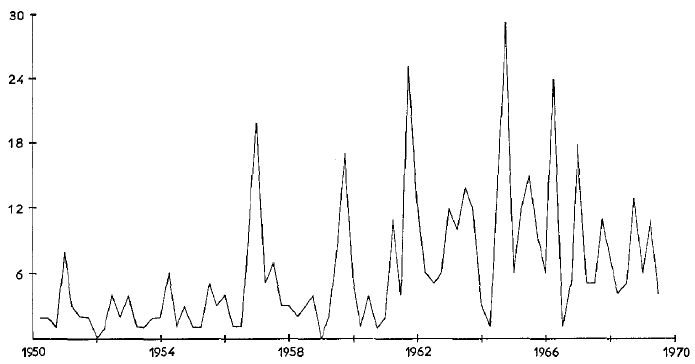
\includegraphics[width=5in]{earthquakes}
	\caption[Number of shocks in periods of three months for area of North Atlantic.]{Number of shocks in periods of three months for area of North Atlantic \cite{thesis}.}
	\label{figure:earth}
\end{figure}